\documentclass[tikz,border=8pt]{standalone}
\usepackage{pgfplots}
\pgfplotsset{compat=1.16}
\begin{document}
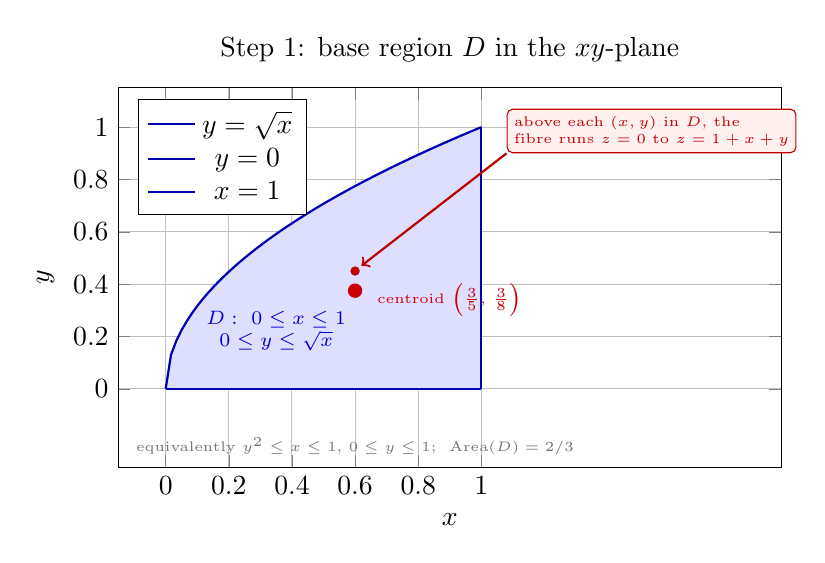
\begin{tikzpicture}
\begin{axis}[
    width=10cm, height=6.4cm,
    xlabel=$x$, ylabel=$y$,
    xmin=-0.15, xmax=1.95, ymin=-0.30, ymax=1.15,
    xtick={0,0.2,...,1}, ytick={0,0.2,...,1},
    grid=major, title={Step 1: base region $D$ in the $xy$-plane},
    legend pos=north west, legend style={fill=white},
    clip=false,
]
\addplot[fill=blue!13, draw=none, domain=0:1, samples=60, forget plot] {sqrt(x)} \closedcycle;
\addplot[thick, blue!70!black, domain=0:1, samples=60] {sqrt(x)};
\addlegendentry{$y=\sqrt{x}$}
\addplot[thick, blue!70!black] coordinates {(0,0) (1,0)};
\addlegendentry{$y=0$}
\addplot[thick, blue!70!black] coordinates {(1,0) (1,1)};
\addlegendentry{$x=1$}
\fill[red!80!black] (axis cs:0.6,0.375) circle (2.6pt);
\fill[red!75!black] (axis cs:0.6,0.45) circle (1.7pt);
\node[font=\tiny, red!80!black, anchor=west] at (axis cs:0.64,0.34) {centroid $\left(\frac{3}{5},\,\frac{3}{8}\right)$};
\draw[->, red!75!black, thick] (axis cs:1.08,0.90) -- (axis cs:0.62,0.47);
\node[draw=red!75!black, fill=red!6, rounded corners=2pt, inner sep=2.5pt,
      font=\tiny, text=red!75!black, align=left, anchor=south west]
      at (axis cs:1.08,0.90) {above each $(x,y)$ in $D$, the\\ fibre runs $z=0$ to $z=1+x+y$};
\node[font=\scriptsize, blue!80!black, align=center] at (axis cs:0.35,0.22)
     {$D:\ 0\le x\le 1$\\ $0\le y\le\sqrt{x}$};
\node[font=\tiny, black!55] at (axis cs:0.6,-0.22)
     {equivalently $y^{2}\le x\le 1$, $0\le y\le 1$; \ Area$(D)=2/3$};
\end{axis}
\end{tikzpicture}
\end{document}
